\paragraph{Часть 1:}
Топология сети:

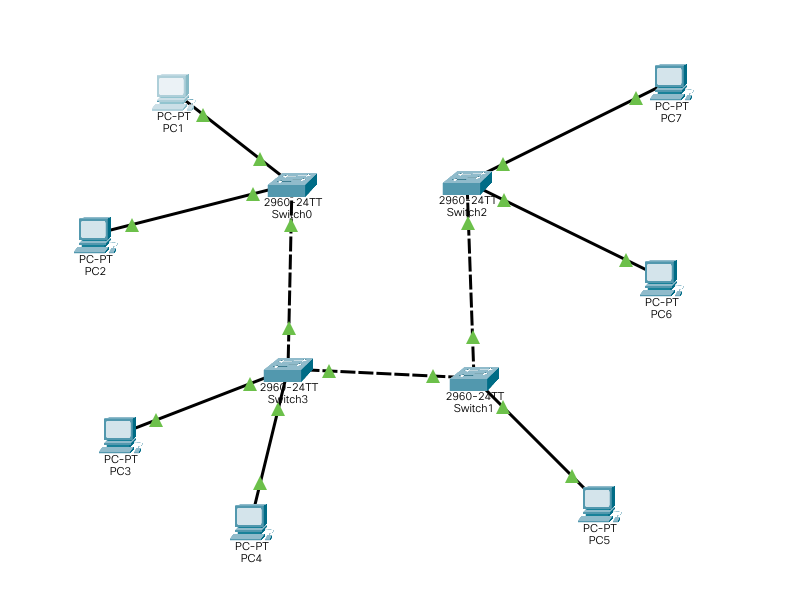
\includegraphics[width=0.9\textwidth]{resources/topology1}

\begin{center}
    \begin{tabular}{|c|c|c|}
        \hline
        Устройство & IP ADDRESS & SUBNET MASK   \\
        \hline
        PC1        & 3.1.1.1    & 255.255.255.0 \\
        PC2        & 3.1.1.2    & 255.255.255.0 \\
        PC3        & 3.1.1.3    & 255.255.255.0 \\
        PC4        & 3.1.1.4    & 255.255.255.0 \\
        PC5        & 3.1.1.5    & 255.255.255.0 \\
        PC6        & 3.1.1.6    & 255.255.255.0 \\
        PC7        & 3.1.1.7    & 255.255.255.0 \\
        \hline
    \end{tabular}
\end{center}

Тесты:
\lstinputlisting[label={lst:resources/pc1}]{resources/pc1}
\lstinputlisting[label={lst:resources/pc2}]{resources/pc4}
